\documentclass[pdftex,letterpaper,12pt]{report}
\usepackage{thesis}
\usepackage{amsmath}
\usepackage{amssymb}
\usepackage{amsthm}
\usepackage{mathtools}
\usepackage{bm}
\usepackage{gensymb}
\usepackage{wasysym}
\usepackage{mathtools}
\usepackage{physics}
\usepackage{empheq}
\usepackage{cases}
\usepackage{rotating}
\usepackage{subfig}
\usepackage{caption}
\usepackage{multirow}
\captionsetup{labelfont=bf} 
\captionsetup[subfloat]{position=top,singlelinecheck=off,justification=raggedright,font=bf,labelfont=large,labelformat=simple,captionskip=-2mm}
\usepackage{float}
\usepackage{enumitem} 
\usepackage[toc,page]{appendix}






\begin{document}
	
\begin{subequations}
	\begin{gather}
	k_{Rb-^{3}He}(T)=55.9(9)\left(\frac{T}{473.15K}\right)^{3.31(12)} {\rm Hz/amg}\\
	k_{Rb-N_{2}}(T)=290(30)\left(\frac{T}{473.15K}\right)^{2.0(25)}{\rm Hz/amg}\\
	k_{Rb-Rb}=4.813(48)\times 10^{-13} {\rm Hz\cdot cm^{3}}
	\end{gather}
\end{subequations}

\begin{subequations}\label{InitialSpinup}
	\begin{gather}
	P_{pc}(t)=\gamma_{se}P_{A}t-\frac{1}{2}\gamma_{se}P_{A}(\gamma_{se}+\Gamma_{pc}+d_{pc})t^{2}\\
	P_{tc}(t)=\frac{1}{2}\gamma_{se}P_{A}d_{tc}t^{2}
	\end{gather}
\end{subequations}

This is a test:
\begin{equation}
L_{AFP}=1-e^{\int \frac{1}{T_{r1}} dt} \approx \int \frac{1}{T_{r1}} dt
\end{equation}
$\gamma /2\pi \approx 3.2434\,{\rm kHz/Gauss}$

\begin{table*}\scriptsize
	\captionsetup{font=scriptsize}
	\begin{center}
		\def\arraystretch{0.75}
		\setlength\tabcolsep{2pt}
		\begin{tabular}{|c|c|c|c|c|c|c|}
			\hline
			Cell Name & Fill Type & Geometry & Glass & Metal & Max Lifetime (hr) & Fill Date\\ \hline
			Tyrion & NGP & Sphere & GE180 & Gold on glass & 1.21 & 6/18/09 \\ \hline
			Gold Maiden1 & NGP & Flange & Pyrex & Gold on Copper & 2.14 & 6/18/10 \\ \hline
			Gold Maiden2 & NGP & Flange & Pyrex & Gold on Copper & None & 8/14/10\\ \hline
			Gold Maiden3 & NGP & Flange & Pyrex & Gold on Copper & 6.49 & 11/11/10\\ \hline
			Goldfinger & NGP & Vertical & Pyrex & Gold on Copper & 3.59 & 4/28/13\\ \hline
			Cupid & NGP & Vertical & Pyrex & Bare Copper & 3.13 & 6/15/13\\ \hline
			Goldeneye & NGP & Vertical with Valve & Pyrex & Gold on Copper & 13.94 & 10/2/13\\ \hline
			GoldRush & NGP & Vertical & Pyrex & Gold on Copper & 14.81$^\dagger$  & 11/8/13\\ \hline
			Pyrah & NGP & Vertical & Pyrex & None & 26.52$^\dagger$ & 2/1/14\\ \hline
			GoldenVec & NGP & Horizontal & Pyrex & Gold on Copper & 10.6 & 10/18/14\\ \hline
			TitanVec & NGP & Horizontal & Pyrex & Gold on Titanium & 0.52 & 12/15/14\\ \hline
			GoldenVec2 & Cryogenic & Horizontal & Pyrex & Gold on Copper & 15.6 & 2/14/15\\ \hline
			Titan & NGP & Vertical & Pyrex & Bare Titanium & None & 3/11/15\\ \hline
			GoldenVec180 & Cryogenic & Horizontal & GE180 & Gold on Copper & 4.43 & 6/17/15\\ \hline
			GolderVec360 & Cryogenic & Horizontal & GE180 & Gold on Copper & 3.01 & 7/11/15\\ \hline
			Tweety & Cryogenic & Vertical & Pyrex & Canary Glass & 22.7 & 9/22/15 \\ \hline
			Sylvester & Cryogenic & Horizontal & GE180 & Canary Glass & 6.39 & 11/20/15\\ \hline
			Kappa1 & Cryogenic & Sphere & GE180 & None & 72.17 & 2/6/16\\ \hline
			Goldfinger180 & Cryogenic & Vertical & GE180 & Gold on Copper & 12.4 $^\dagger$ & 5/19/16\\ \hline
		\end{tabular}
		\caption
		{Shown are the fill information, design and maximum measured lifetime of the test cells. Fill type is the method of cleaning gas filled into the cell. $^\dagger$ indicates the maximum lifetime was obtained at an elevated position. Although canary glass is not metal, it is listed in the column of metal for Tweety and Sylvester for the sake of convenience.}
		\label{test_cells}
	\end{center}
\end{table*}

\begin{center}
	\begin{tabular}{ | c | c| c| c | }
		\hline
		& turns & radius & separation \\ \hline
		x & 42 & 33 cm & 64 cm \\ \hline 
		y & 100 & 28 cm & 56 cm \\ \hline
		z & 8 & 66 cm & 66 cm \\
		\hline
	\end{tabular}
\end{center}

\begin{figure}[t!]
	\centering
	\resizebox{0.6\textwidth}{!}{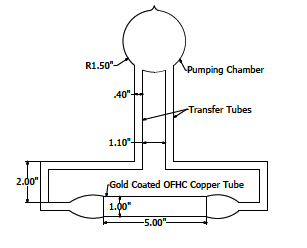
\includegraphics{goldenvec.png}}
	\caption{{Design of the horizontal cell GoldenVec.}}
	\label{goldenvec}
\end{figure}

\begin{figure}[t!]
	\centering
	\resizebox{0.91\textwidth}{!}{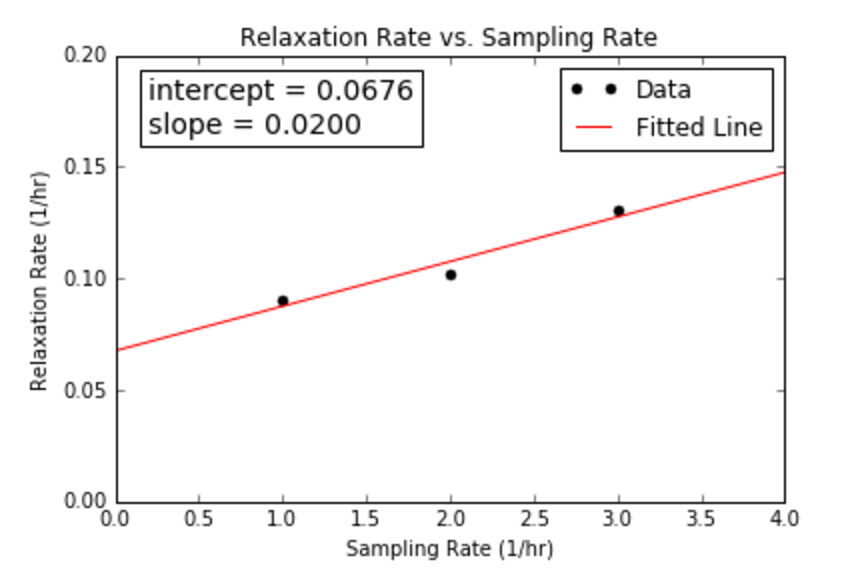
\includegraphics{corrected_T1.png}}
	\caption{{A linear fit to extract lifetime corrected for relaxation due to PNMR losses.}}
	\label{corrected_T1}
\end{figure}

See in Fig.~\ref{spinup}


	
The energy levels of $^{87}$Rb are shown in Fig.~\ref{fig:foms}.
where $\Gamma_{A}$ is the pressure dependent FWHM, $\Gamma_{A}\approx 0.04nm/amg \cdot [^{3}He]$.

\addcontentsline{toc}{chapter}{Bibliography}
\bibliography{ref}

\end{document}